\section{Annotation of the QuadTrack Dataset}

%

In the annotation process of the established QuadTrack dataset, we used CVAT~\cite{cvat}, an open-source annotation tool that supports tasks such as object detection, object tracking, and instance segmentation. CVAT offers both local and online versions, providing high flexibility for users. 
Prior to annotation, we preprocessed the dataset by selecting representative scenes, including $32$ sequences (seq), with $16$ sequences allocated for training and $16$ for testing. 
Each sequence contains $600$ frames with a frame rate of approximately $10$FPS, resulting in a duration of about $60$ seconds per sequence. 
Furthermore, to assist annotators in better semantic understanding and precise labeling, we unfolded the images into a $2048{\times}480$ panoramic layout via equirectangular projection. 
For the bounding boxes at the image borders, we ensured continuous tracking, guaranteeing that the same object in the surrounding environment maintained a unique ID. The minimum bounding box area was set to $800$ pixels, and any targets smaller than this area were ignored. 
The QuadTrack dataset includes two common object classes: \emph{car} and \emph{person}.

Upon completion of the annotation process, the final annotation attributes were thoroughly reviewed and validated through a filtering and cross-validation procedure to ensure data accuracy. After ensuring the correctness of the annotations, the final annotation attributes were formatted into the MOT standard~\cite{milan2016mot16}. 
%
Example of ground truth:


\begin{lstlisting}[language={Python}]
# MOT format
# f_id, t_id, x, y, w, h, conf, cls, vis
# data
1,1,733.67,281.66,34.78,106.81,1,1,1.0
1,2,557.87,268.05,24.36,128.58,1,1,1.0
1,3,382.33,316.41,110.61,61.49,1,2,1.0
1,4,000.00,301.35,35.02,82.89,1,2,1.0
1,5,1917.7,278.79,20.70,97.98,1,1,1.0
...
\end{lstlisting}


For a comprehensive description of the attributes in the dataset, please refer to Tab.~\ref{tab:anno}.
This annotation format, commonly used in Multi-Object Tracking (MOT) research, provides a structured and standardized method for organizing the data. 
%
The inclusion of essential attributes such as object identity, bounding box coordinates, and visibility status is critical for training and assessing tracking models in dynamic, real-world environments. 
In Fig.~\ref{fig:vis_anno}, examples from the QuadTrack dataset are shown, demonstrating the diversity of scenes and the visual presentation of annotations.

\begin{figure}[!t]
  \centering
  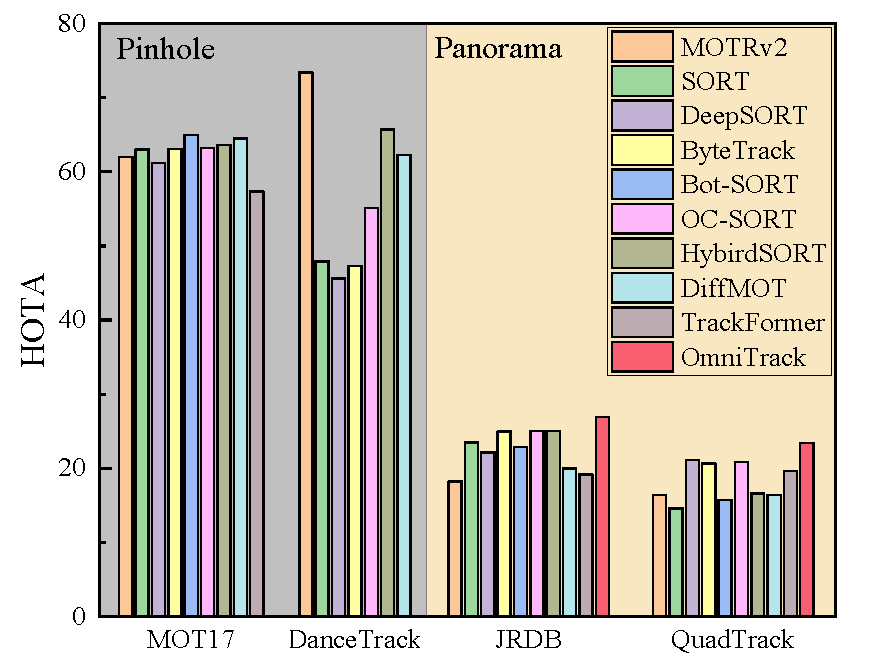
\includegraphics[width=0.48\textwidth]{imgs/SOTA_v2.pdf}
  %\vskip -2ex
  \caption{Comparison of state-of-the-art methods on different datasets. \textbf{Pinhole} refers to Multi-Object Tracking (MOT) datasets that utilize pinhole camera images, whereas \textbf{Panorama} refers to MOT datasets that employ panoramic images.}
  \label{fig:SOTA}
  %\vskip -2ex
\end{figure}

\begin{table*}[t!]
    \centering
    \setlength{\tabcolsep}{16pt}     % 4pt
    % \resizebox{\columnwidth}{!}{%
    \small
    \begin{tabular}{lll}
        % \toprule
        \topline
        \rowcolor{mygray}  Pos. & {Key} &  Explanation  \\
        % \midrule
        \hline
        1 & Frame\_id & Represents the frame ID. \\
        2 & Track\_id & A unique identifier for each object. A value of -1 indicates a detection item. \\
        3 & Left & Coordinates of the top-left corner of the object bounding box. \\
        4 & Top & Coordinates of the top-left corner of the object bounding box. \\
        5 & Width & Width of the object bounding box. \\
        6 & Height & Height of the object bounding box. \\
        7 & Confidence & It acts as a flag whether the entry is to be considered (1) or ignored (0). \\
        8 & Class & Indicates the type of object annotated. \\
        9 & Visibility & Visibility ratio, a number between 0 and 1 that says how much of that object is visible.\\
        % \bottomrule
        \bottomline
    \end{tabular}
    % }
    \vspace{-1mm}
    \caption{Detailed explanation of the annotation attributes for the QuadTrack dataset, including the meaning of each position.}
    \vspace{-3mm}
    \label{tab:anno}
\end{table*}


\begin{figure*}[!t]
  \centering
  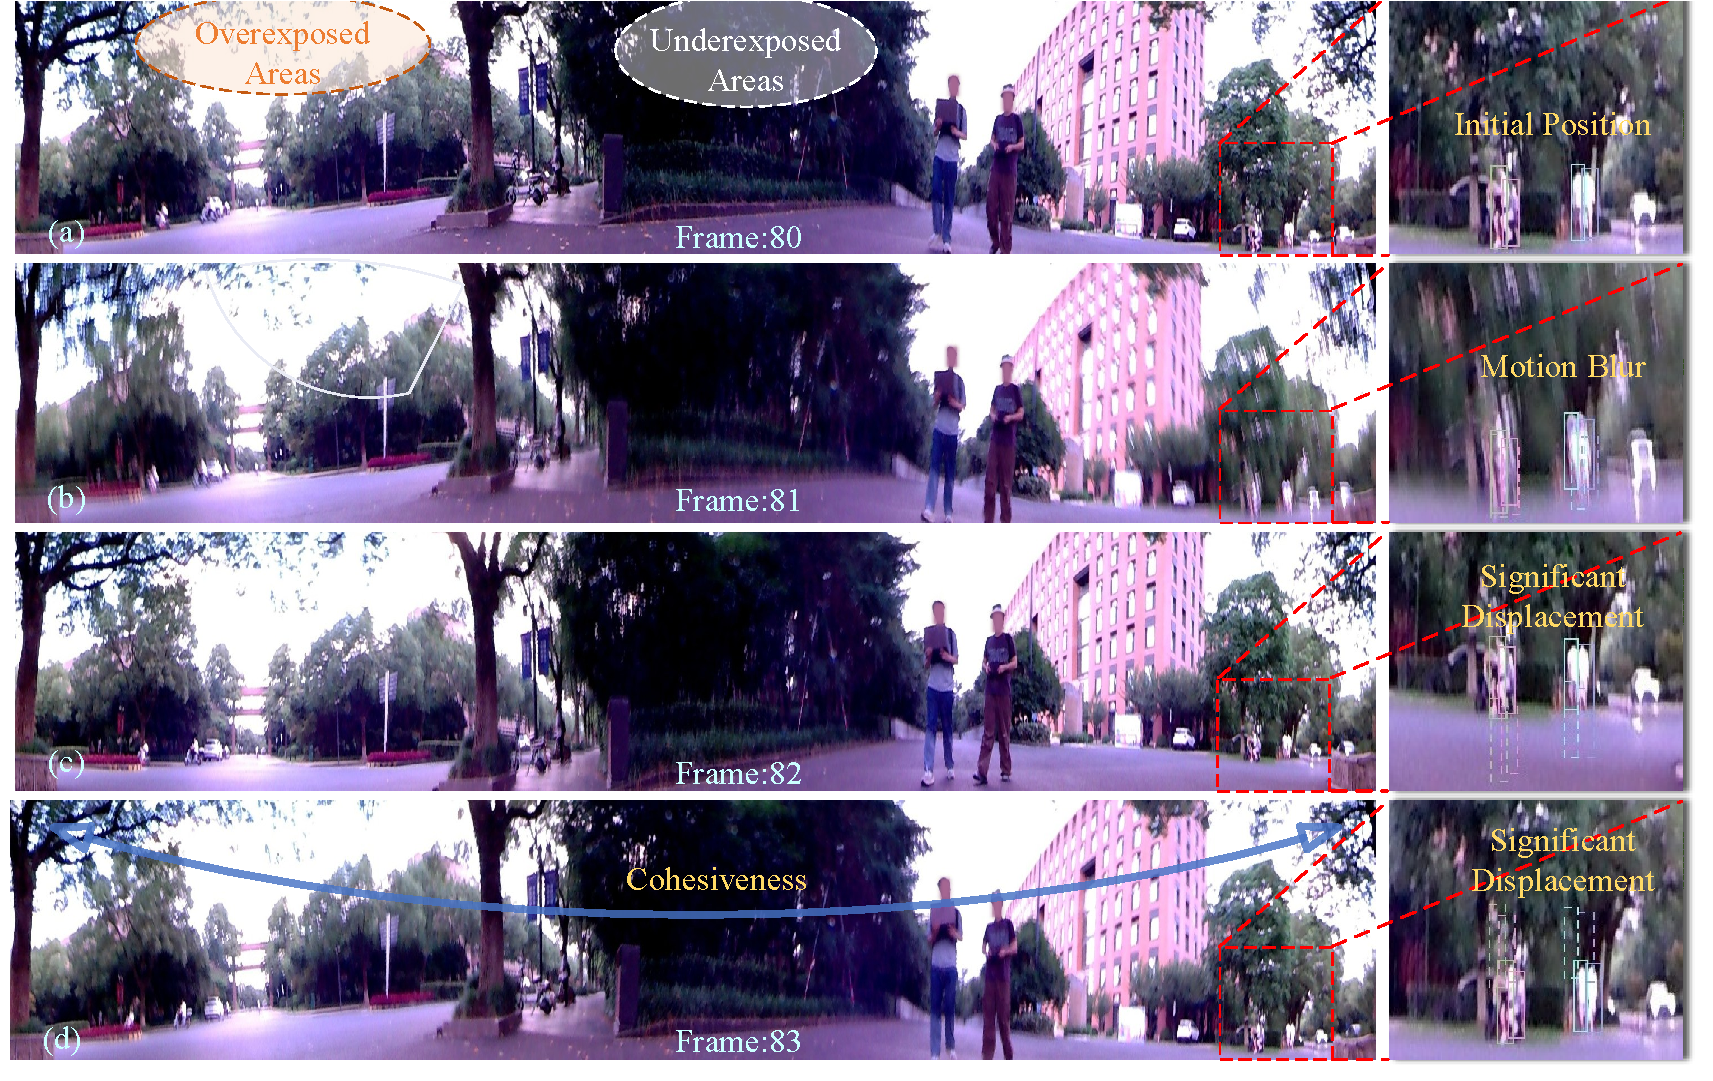
\includegraphics[width=0.95\textwidth]{imgs/quadtrack_challenge_v1.pdf}
  %\vskip -2ex
  \caption{The QuadTrack dataset presents several significant challenges. The images labeled (a), (b), (c), and (d) illustrate continuous frames $80$ to $84$ from a sequence, with corresponding magnified views shown on the right. In these magnifications, solid rectangular boxes represent the Ground Truth (GT) for the current frame, while dashed boxes correspond to the GT from the preceding frame. One notable challenge is motion blur, particularly evident in the magnified view of frame (b), where the bionic gait introduces substantial blur to the target object. Moreover, there is considerable positional displacement between adjacent frames, as demonstrated in the magnified views of frames (c) and (d). The panoramic images also present inherent exposure issues, displaying both overexposed and underexposed regions, as seen in (a). Finally, the continuity inherent in the panoramic images presents an additional critical factor for the tracking task.}
  \label{fig:challenge}
  %\vskip -2ex
\end{figure*}
